\articlepart{タイピングとキーボード}{eigh}

\section{はじめに}
タイパーにとってキーボードと言ったらどんな存在でしょうか。キーボードはタイピングにおいて必要不可欠な道具であり、タイピングに大きな影響を与えています。しかし、キーボードとタイパーの関係というのは人によって様々だと思います。「キーボードを変えて新記録を出しても実力が伸びたわけじゃないからキーボードを替えたくない」という人や「記録が伸びるならキーボードを替える」という人、「いろんなキーボードの打鍵感を楽しみたい」などいろいろな人がいると思います。 今回はキーボードがタイピングの速さにどのように関わっているかを簡単な実験や主観を交えながら考えていきたいと思います。

\section{タイピングにおけるキーボード}

\subsection{なぜキーボードにこだわるか}
どのタイパーも、程度の違いはあれキーボードを替えることによりタイピングの速さは変わります。また、タイピングの速さだけでなく成長速度にも影響しているようで、キーボードを替えたことによって記録が伸びたタイパーも少なくありません。ではキーボードのどのような要素がタイピングの速さに影響を与えているのでしょうか。

\subsection{タダの入力機器なのか?}
キーボードを物理的な側面から捉えると、各キーごとのスイッチによってPCへ電気信号を入力する機器と見ることができます。この関係をシンプルに表現すると図\ref{eigh:img1}のようになります。しかし、このような一方通行の関係では、タイピングに与えている影響を読み取ることができません。現実にタイピングの速さ(言い換えるとタイパーの打鍵動作)に大きく影響していることを考えると、キーボード自体がタイパーにもなんらかのフィードバックを行っている「タイパーへの入力装置」としての働きがあると考えることができます。これを示したのが図\ref{eigh:img2}になります。

\begin{figure*}
 \begin{center}
   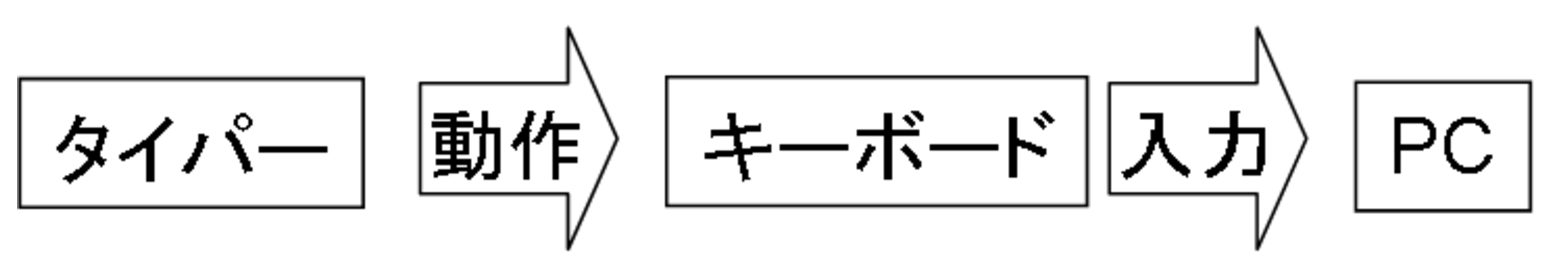
\includegraphics[width=14cm,clip]{res_eigh/img1.eps}
 \end{center}
 \caption{タイパーとキーボード、PCとの関係}
 \label{eigh:img1}
\end{figure*}

\begin{figure*}
 \begin{center}
   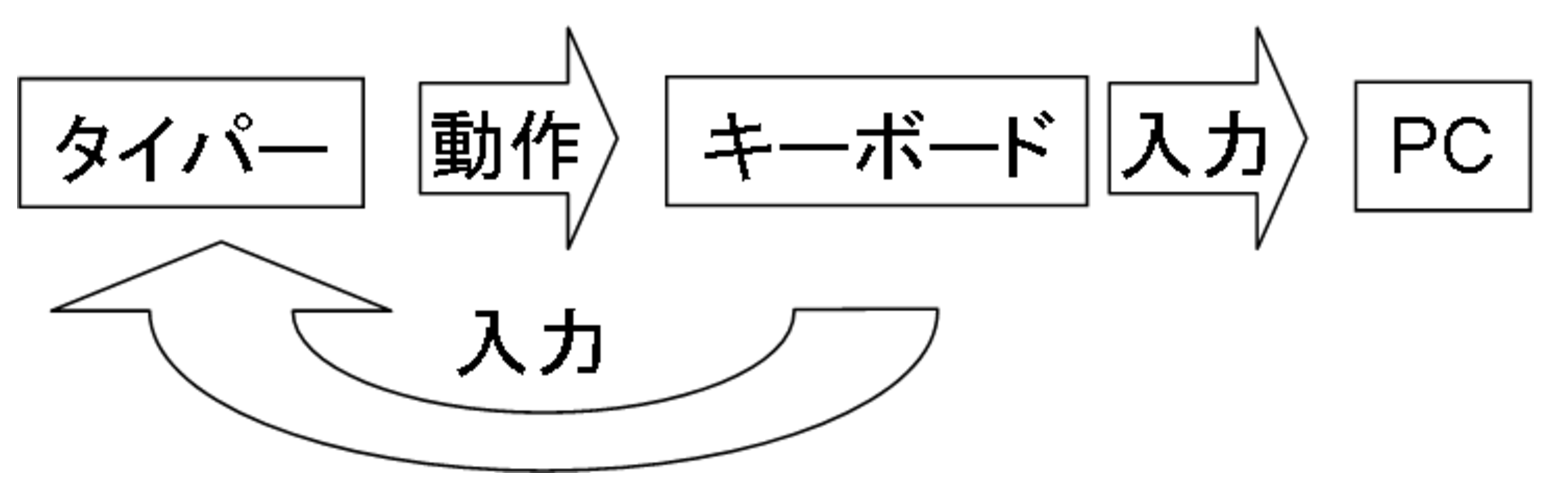
\includegraphics[width=14cm,clip]{res_eigh/img2.eps}
 \end{center}
 \caption{キーボードからタイパーへの「入力」}
 \label{eigh:img2}
\end{figure*}

タイピング中は、キーボードはタイパーからPCへキー情報を入力するだけでなくタイパーへも多くの情報を入力し、タイピングに影響していると考えられます。

\subsection{キーボードからの情報}

ではタイピング中にどのような情報が入力されるのでしょうか。五感の中でキーボードに関係するのは主に聴覚と触覚です。音の情報も重要だとは思いますが、やはりキーボードから得られる情報で重要な要素は触覚情報、つまりキーの反発の仕方であると考えます。では具体的にキーボードの荷重特性\footnote{簡単にいえばキーを押すにはどれくらいの力が必要か、という特徴。キーボードやその構造によって大きく異なる。}を見ることで、反発のどのような要素がタイパーへの入力と解釈できるか詳しく見てみます。

\subsection{一般的なキーボードの荷重特性}

キーボードの特徴を表現するために荷重特性というグラフがよく用いられます。一般的なキーボードの荷重特性から見てみましょう。図\ref{eigh:img4}は一般的なラバードーム\footnote{半球状のゴム製の部品}を使用したキーボードにおける荷重特性のグラフです。実際にこのような荷重特性を持つキーボードがあるというわけではありませんが、多くのキーボードでこのようなグラフを描きます。横軸はキーを押した深さ、縦軸はキーボードからの反発力を表しています。

\begin{figure*}
 \begin{center}
   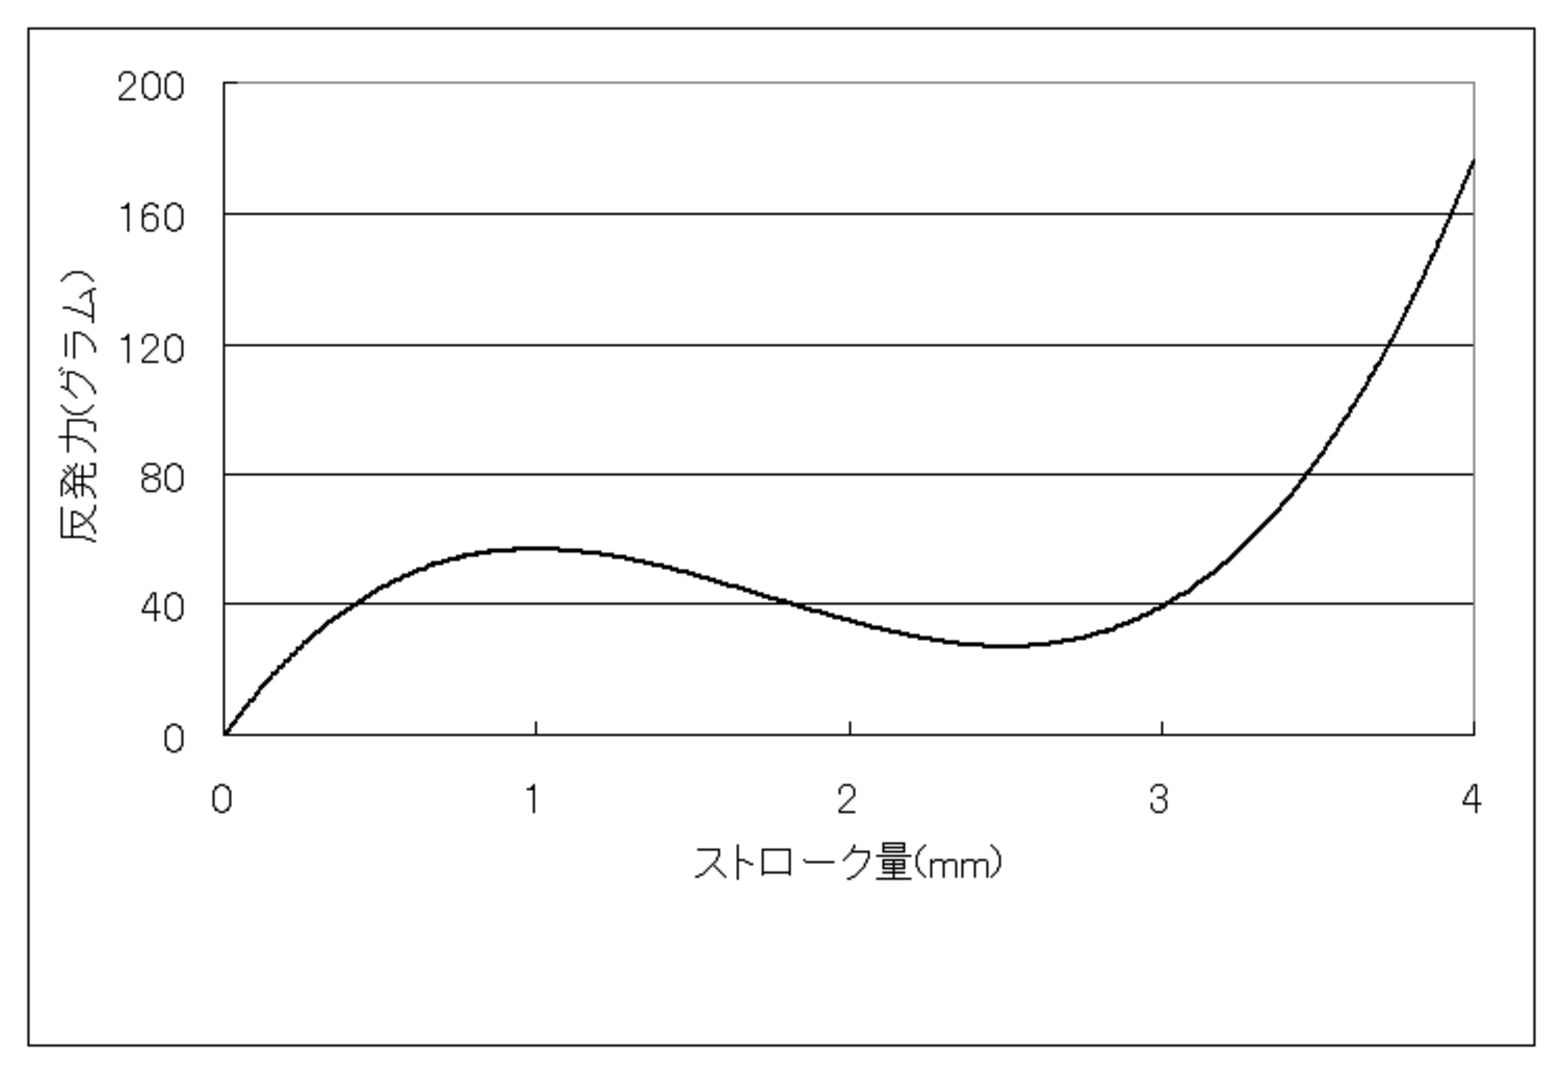
\includegraphics[width=14cm,clip]{res_eigh/img4.eps}
 \end{center}
 \caption{キーボードの荷重特性}
 \label{eigh:img4}
\end{figure*}

このグラフの特徴を右に進みながら見てみましょう。まず、ある点まで反発力が増加していき、そこを頂点に減少しはじめます。ある点まで減少が続き、再び増加へと転じます。最後は値がどんどん大きくなっていきます。とりあえずここでは最初の頂点を「山」、次に一番低くなる場所を「谷」、最後に急激に重さが増える点を「壁」と呼ぶことにします。一般的にキーボードのスペックとして荷重の重さとストロークの深さが書かれていることがありますが、その二つはここでいう山の高さと壁までの距離、ということになります。これらを示したものが図\ref{eigh:img5}になります。

\begin{figure*}
 \begin{center}
   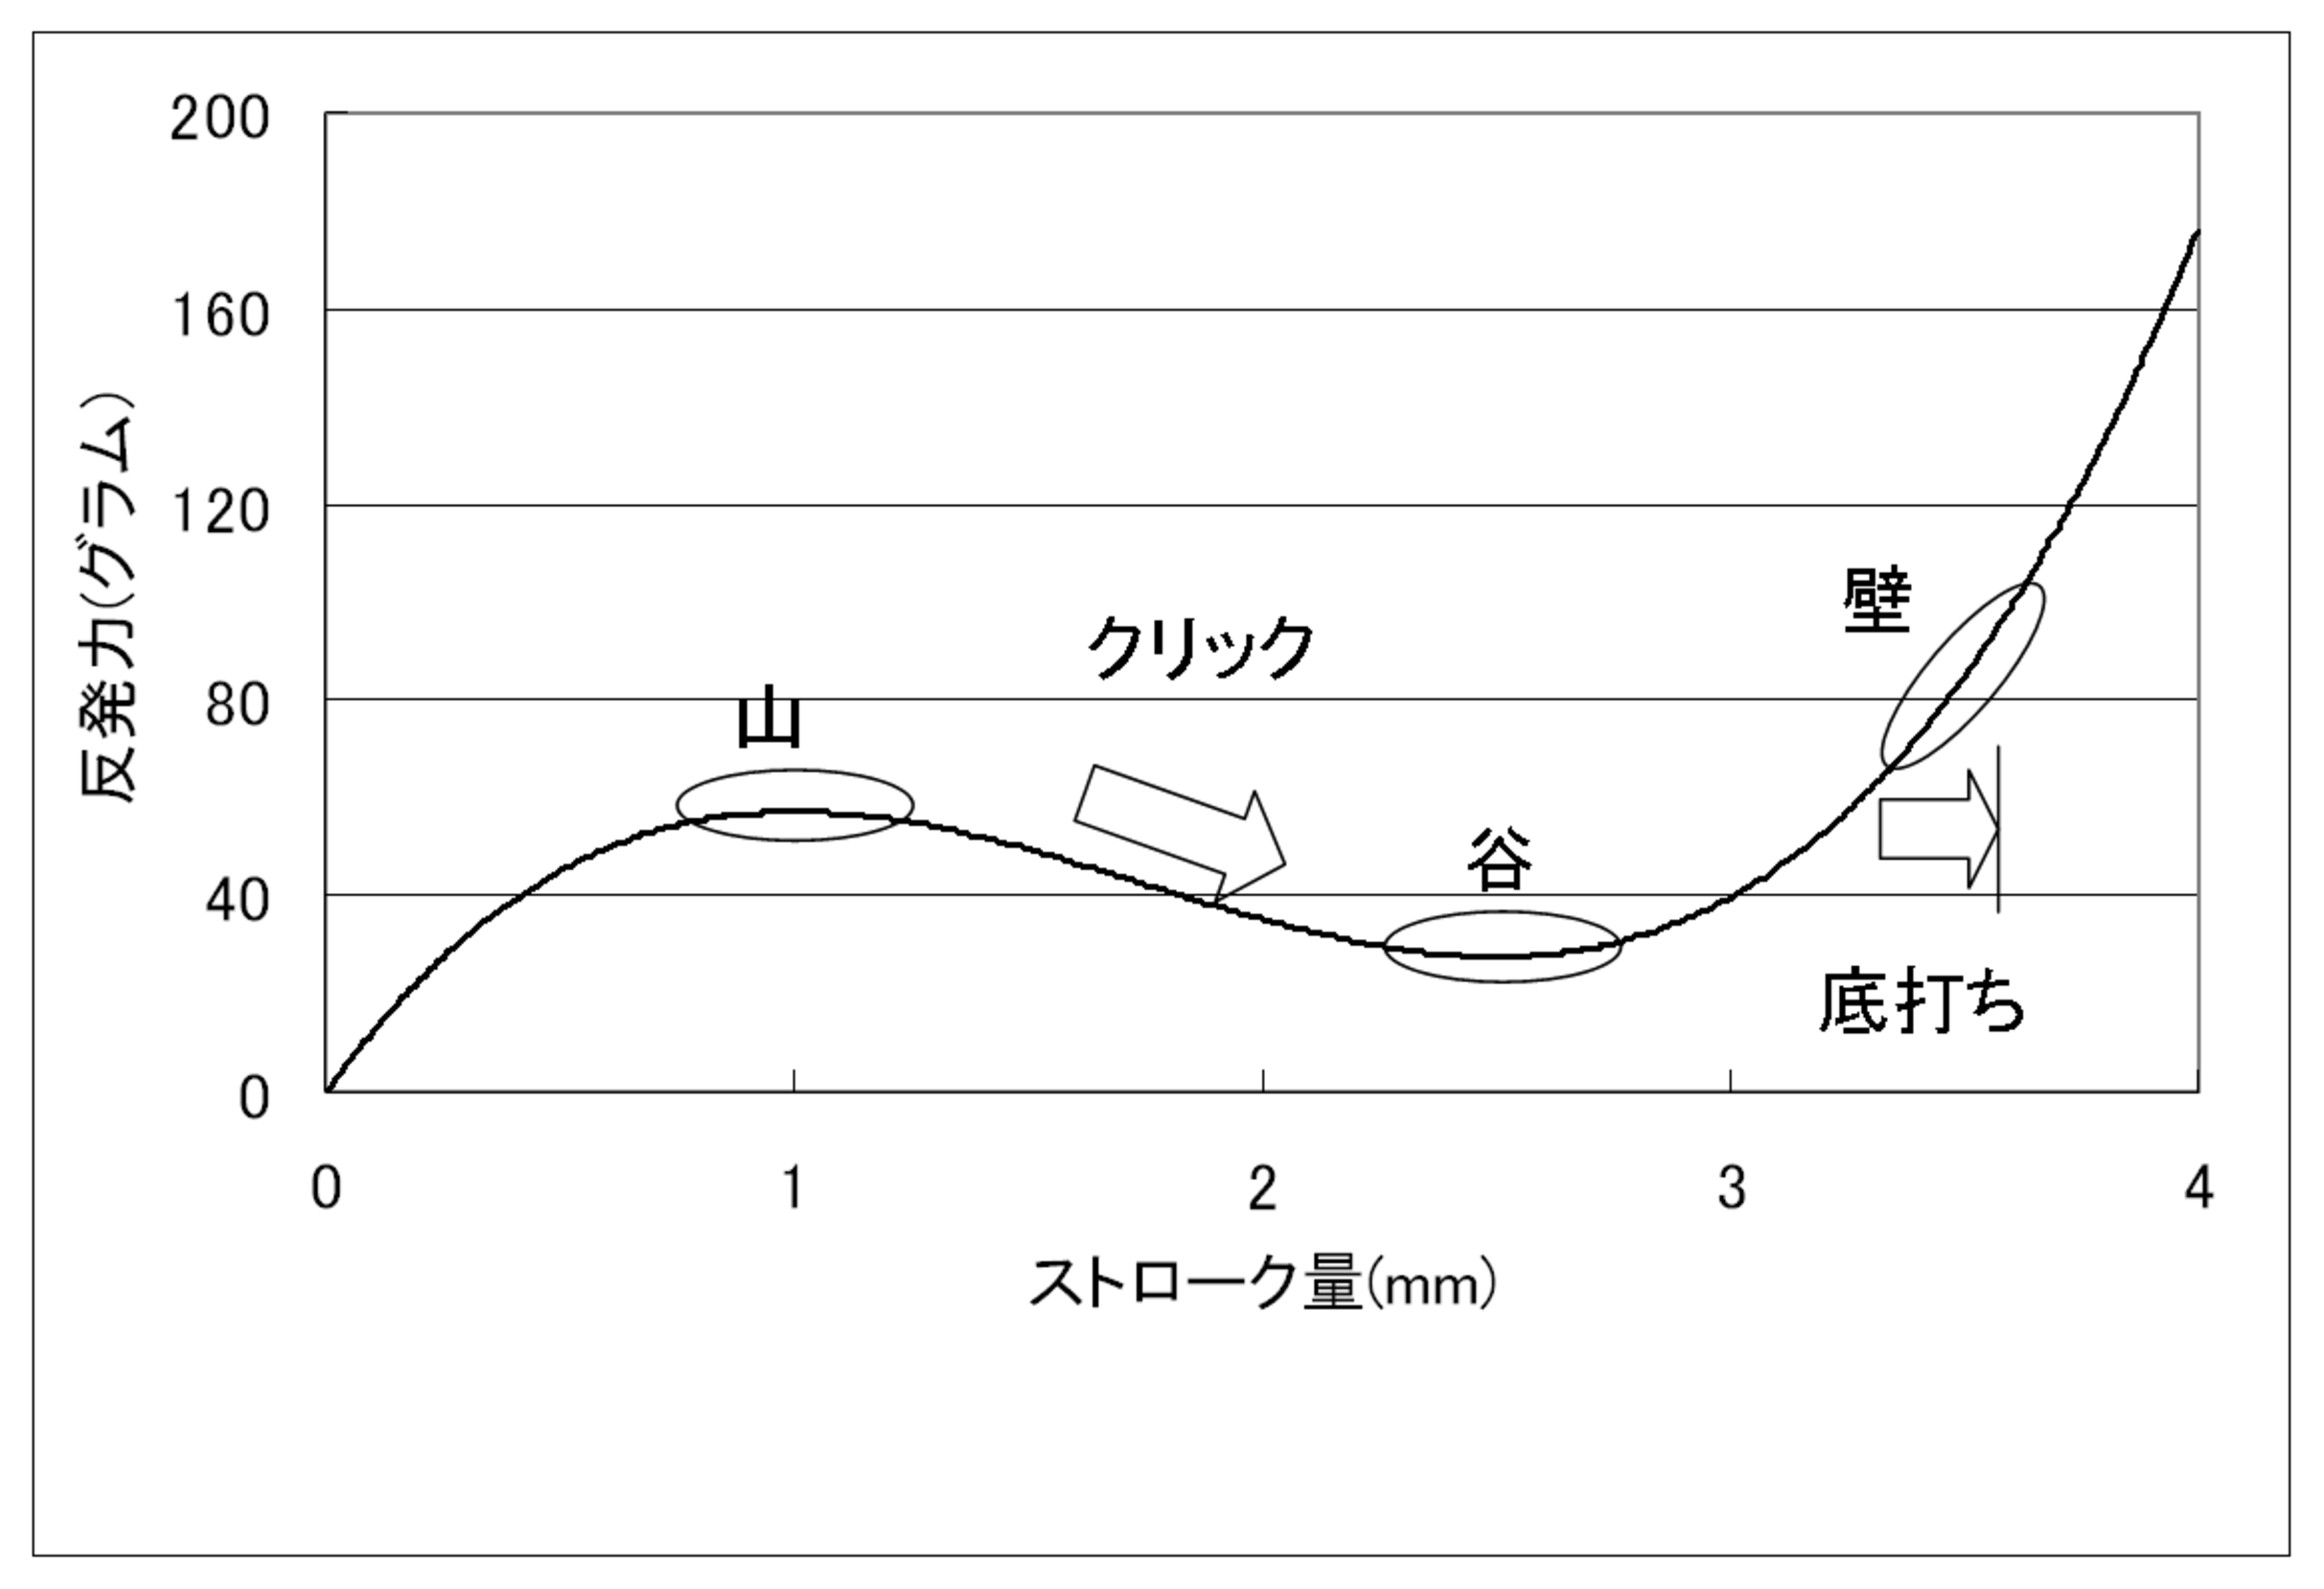
\includegraphics[width=14cm,clip]{res_eigh/img5.eps}
 \end{center}
 \caption{荷重特性とキーボードの入力}
 \label{eigh:img5}
\end{figure*}

\subsection{どの部分を入力とするか}
キーボードの打鍵感について、「クリック感」と「底打ち感」という言葉がよく使われます。クリック感というのは山から谷へかけての部分で、この差が大きい物がクリック感が強いとかはっきりしていると言われます。また、底打ち感を感じるのは壁の部分で、グラフの傾きが大きい(急激に変化している)ものほど底打ち感がはっきりしていると言われます。この「クリック感」「底打ち感」両方に言えることは、傾きが大きいほどはっきり感じるということです。この傾きが一種の入力となっているといっていいでしょう。今回はこれら2つを「クリック」「底打ち」と呼び、キーボードからの「入力」として扱うことにします。

\section{「速い」キーボードの特徴}
「クリック」や「底打ち」という入力に要する時間や感触の強さはキーボードによって、大きく異なります。実際に速く打てると言われているキーボードの特徴を考え、入力がどのようにタイピングの速さに影響しているか見てみましょう。
速く打てるキーボードと言っても人によって相性があったり慣れの問題もあるため一概には言えませんが、タイパーによく使われているキーボードとしては東プレのリアルフォース(リアフォ)とパンタグラフ式のキーボード(パンタ)が挙げられます。この2つのキーボードはどちらも反発が軽い、ストロークが浅いという特徴を持っています。これらの特徴についてキーボードからの入力の時間、強さという観点から考えてみます。

\subsection{入力に要する時間}

\begin{figure*}
 \begin{center}
   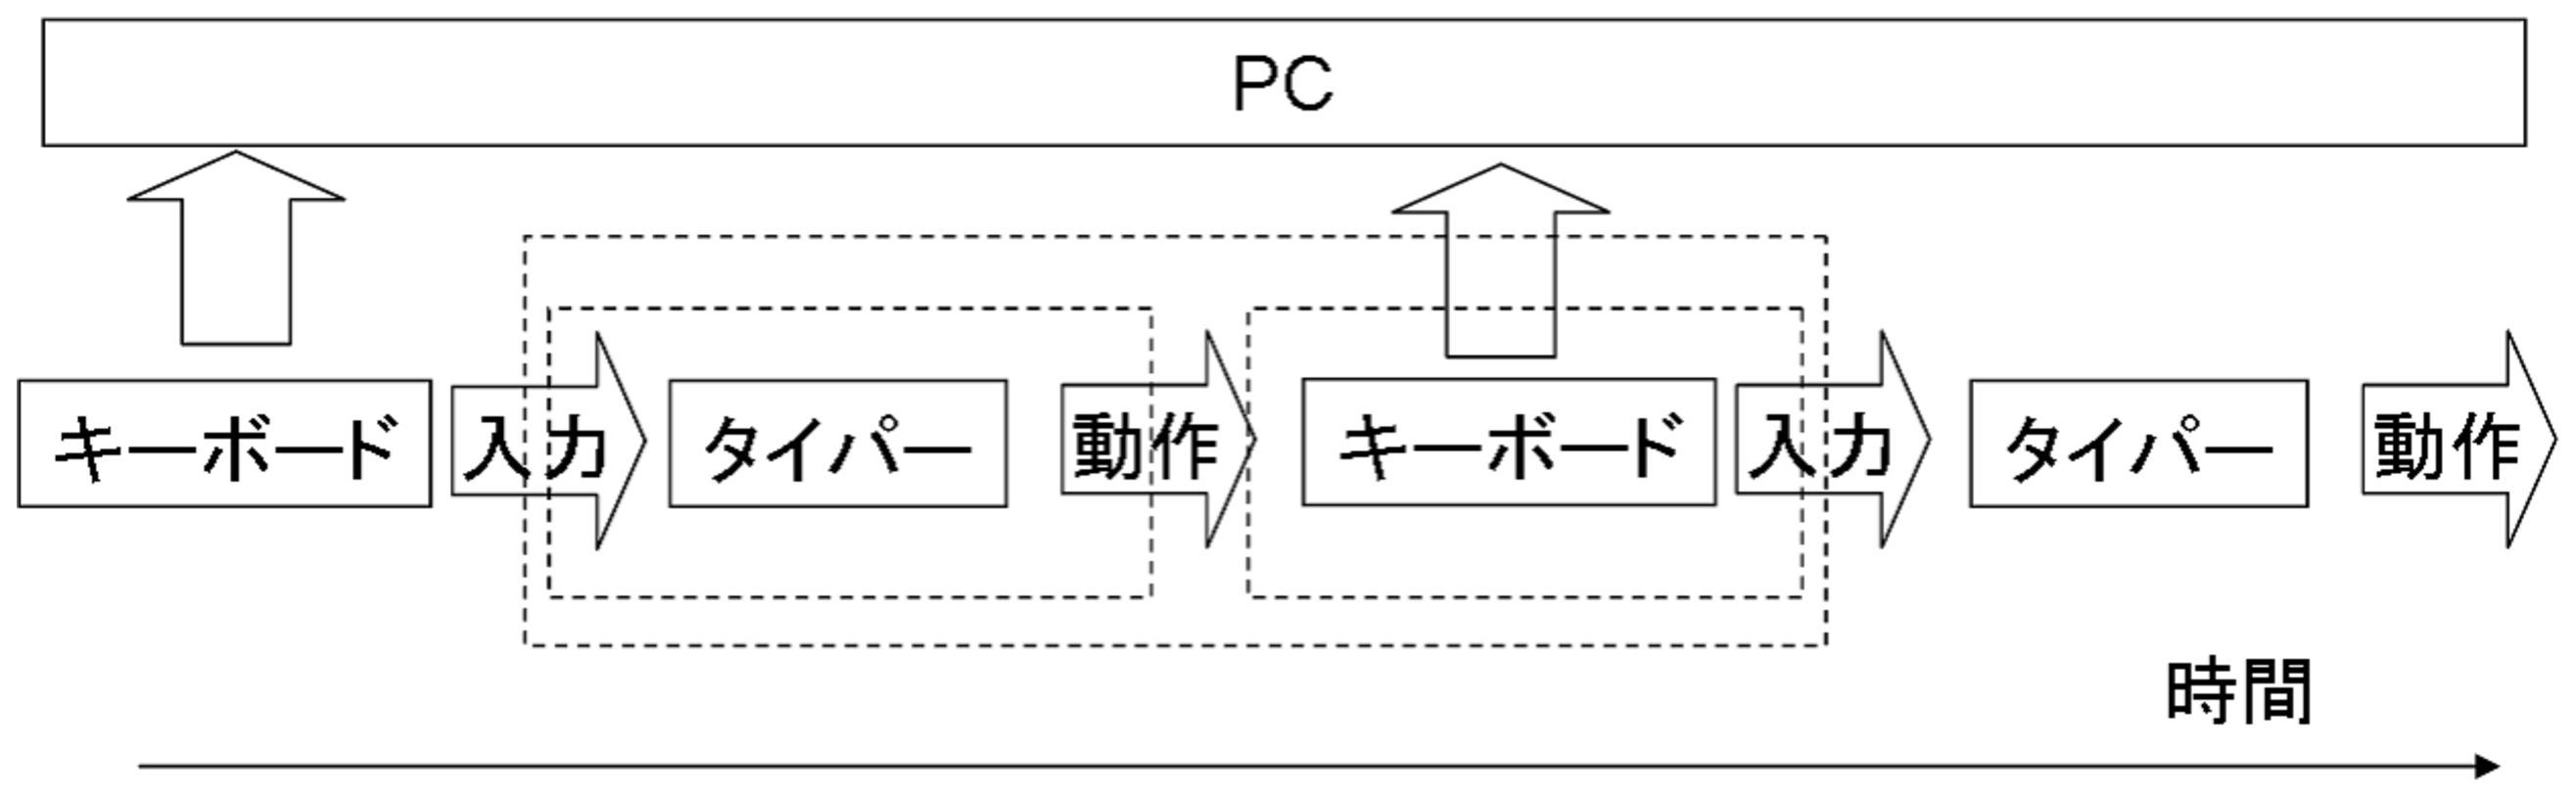
\includegraphics[width=14cm,clip]{res_eigh/img3.eps}
 \end{center}
 \caption{タイパーとキーボードの時間軸上の流れ}
 \label{eigh:img3}
\end{figure*}

図\ref{eigh:img3}のような時間軸上でキーボードとタイパーの相互の影響を見てみると、タイパーが動作を行うことでキーボードの反発の仕方が変わり、それが再びタイパーへの入力になるという流れになります。タイピング中は、タイパーの動作とキーボードからの入力が繰り返されることから、このループの周期が短くなるほどタイピングが速くなります。つまり、タイパーの反応速度(入力から動作までの時間)だけでなく、キーボードの反応時間(タイパーの動作からタイパーへ入力するまでの時間)もタイピングの速さに関係しているということです。この反応時間がキーボードによって異なることから、結果的にキーボードによってタイピングの速さに差が生まれます。ここでは、「タイパーの動作開始」から「クリック入力」までの1サイクルを「反応時間」としています。


\subsubsection*{実験}
キーボードの反応時間は「キーボードの荷重特性」と「キーを押す強さ(速さ)」によって変わります。ここでは、異なる荷重特性を持つ仮想キーボードを用意し、一定の強さでキーを押し込んでいった際の反応時間を計算で求めることで、キーボードの特徴をよりわかりやすく示します。この実験では、基準となるキーボード(基準)、浅いキーボード(浅い)、軽いキーボード(軽い)の3種類の荷重特性(ある位置$x$における反発力の関数)を用意しました。

まず計算方法の説明ですが、キーを押す強さと反発力からキーが押し込まれていく速度が決まり、そこからある時刻のキーの位置やクリックが発生するまでの時間を求めることができます。これらをまとめたものが次の運動方程式になります。高校物理で習った方も(そしてすでに忘れている方も)いらっしゃると思いますが、$F=ma$という運動の公式を使っています。

\[
v(t+1)= v(t) + \frac{F(x)-R(x)}{m}
\]

\noindent $v(t)$:時刻tにおけるキーの速度$[m/s]$ \\
\noindent $F(x)$:位置($x$)におけるキーを押す力(谷までは一定の力、谷に到達したあとは0)$[N]$ \\
\noindent $R(x)$:位置($x$)におけるキーの反発力$[N$] \\
\noindent $m$:指の質量(定数)$[kg]$ \\

\[
x(t+1) = x(t+1) + v(t)
\]
\noindent $x(t)$:時刻$t$におけるキーを押し込んだ位置 $[m]$
 \\

初期値としてキーを押す力$F$、反発力$R$、質量$m$を決めたのちに時刻$t$を徐々に動かしていき、位置$x$が「クリック」「底打ち」「戻り」に到達する時刻を求めます。計算式でイメージしづらい方は以下の流れをご覧下さい。この実験では位置X1、X3、X0に到達するまでの時間を求めます。

\begin{enumerate}
 \item 位置X0:一定の強さで押しはじめる(位置によって反発力が変化していく)
 \item 位置X1:「クリック」に到達する
 \item 位置X2:「谷」に到達する(押す力を0にする)
 \item 位置X3:「底打ち」に到達する
 \item 反発力でキーが戻っていく
 \item 位置X0:「戻り」に到達する
\end{enumerate}

今回は反発力Rの山を「基準」と「浅い」で55g、「軽い」で44gとしました。実験で使った値は荷重特性のグラフのように複雑に変化させていますが、ここでは特徴的な値のみとさせていただきます。また、それぞれの到達位置は「基準」と「軽い」で山、クリック、谷、底打ちの順に、1mm、1.75mm、2.5mm、3.9mmとし、「浅い」は前者を1.4で割った値としました。キーを押す力は102gです。

上記のようなパラメータで実験したところ、表\ref{eigh:result}のような結果が得られました。基準キーボードに対して浅いキーボードは全ての位置に短い時間で到達しています。一方、軽いキーボードではクリックと底打ちまでの時間は短くなっていますが、反発力が弱いために戻るのに余計に時間を要しています。この結果は、軽いキーボードでは同一キーの連打や同じ指を連続で使用する場合に遅くなってしまう可能性があることを示しています。

\begin{table}
\begin{center}
\caption{実験結果}
\label{eigh:result}
\begin{tabular}{|c|c|c|c|}
\hline
 & \multicolumn{3}{|c|}{時間 [ms]} \\
\hline
キーボード & クリック & 底打ち & 戻り \\
\hline
基準 & 25 & 43 & 82 \\
\hline
軽い & 24 & 40 & 83 \\
\hline
浅い & 21 & 36 & 68 \\
\hline
\end{tabular}
\end{center}
\end{table}

\subsection{入力の強さ}
キーボードからの入力に反応してタイピングの動作を行なっていく場合だけでなく、図\ref{eigh:img6}のようにキーボードからの入力を無視して打つような場合もあると思います。このような打ち方をする場合はキーボードからの入力(クリック感や底打ち感)は弱いほうが反応を無視しやすく、打つのが容易になります。

これまで筆者が打ってきたキーボードの中で、入力が弱いキーボードとしてはリアフォとCHERRY社の赤軸スイッチを使用したメカニカルキーボードが挙げられます。これらのキーボードと一般的なもののキーボードの荷重特性を比べた結果が図\ref{eigh:img7}になります。山から谷にかけての変化が小さかったり谷がまったくなかったりしています。筆者の経験では、このような入力が弱いキーボードでは「邪魔されないで打てる」という感覚があります。

\begin{figure*}
 \begin{center}
   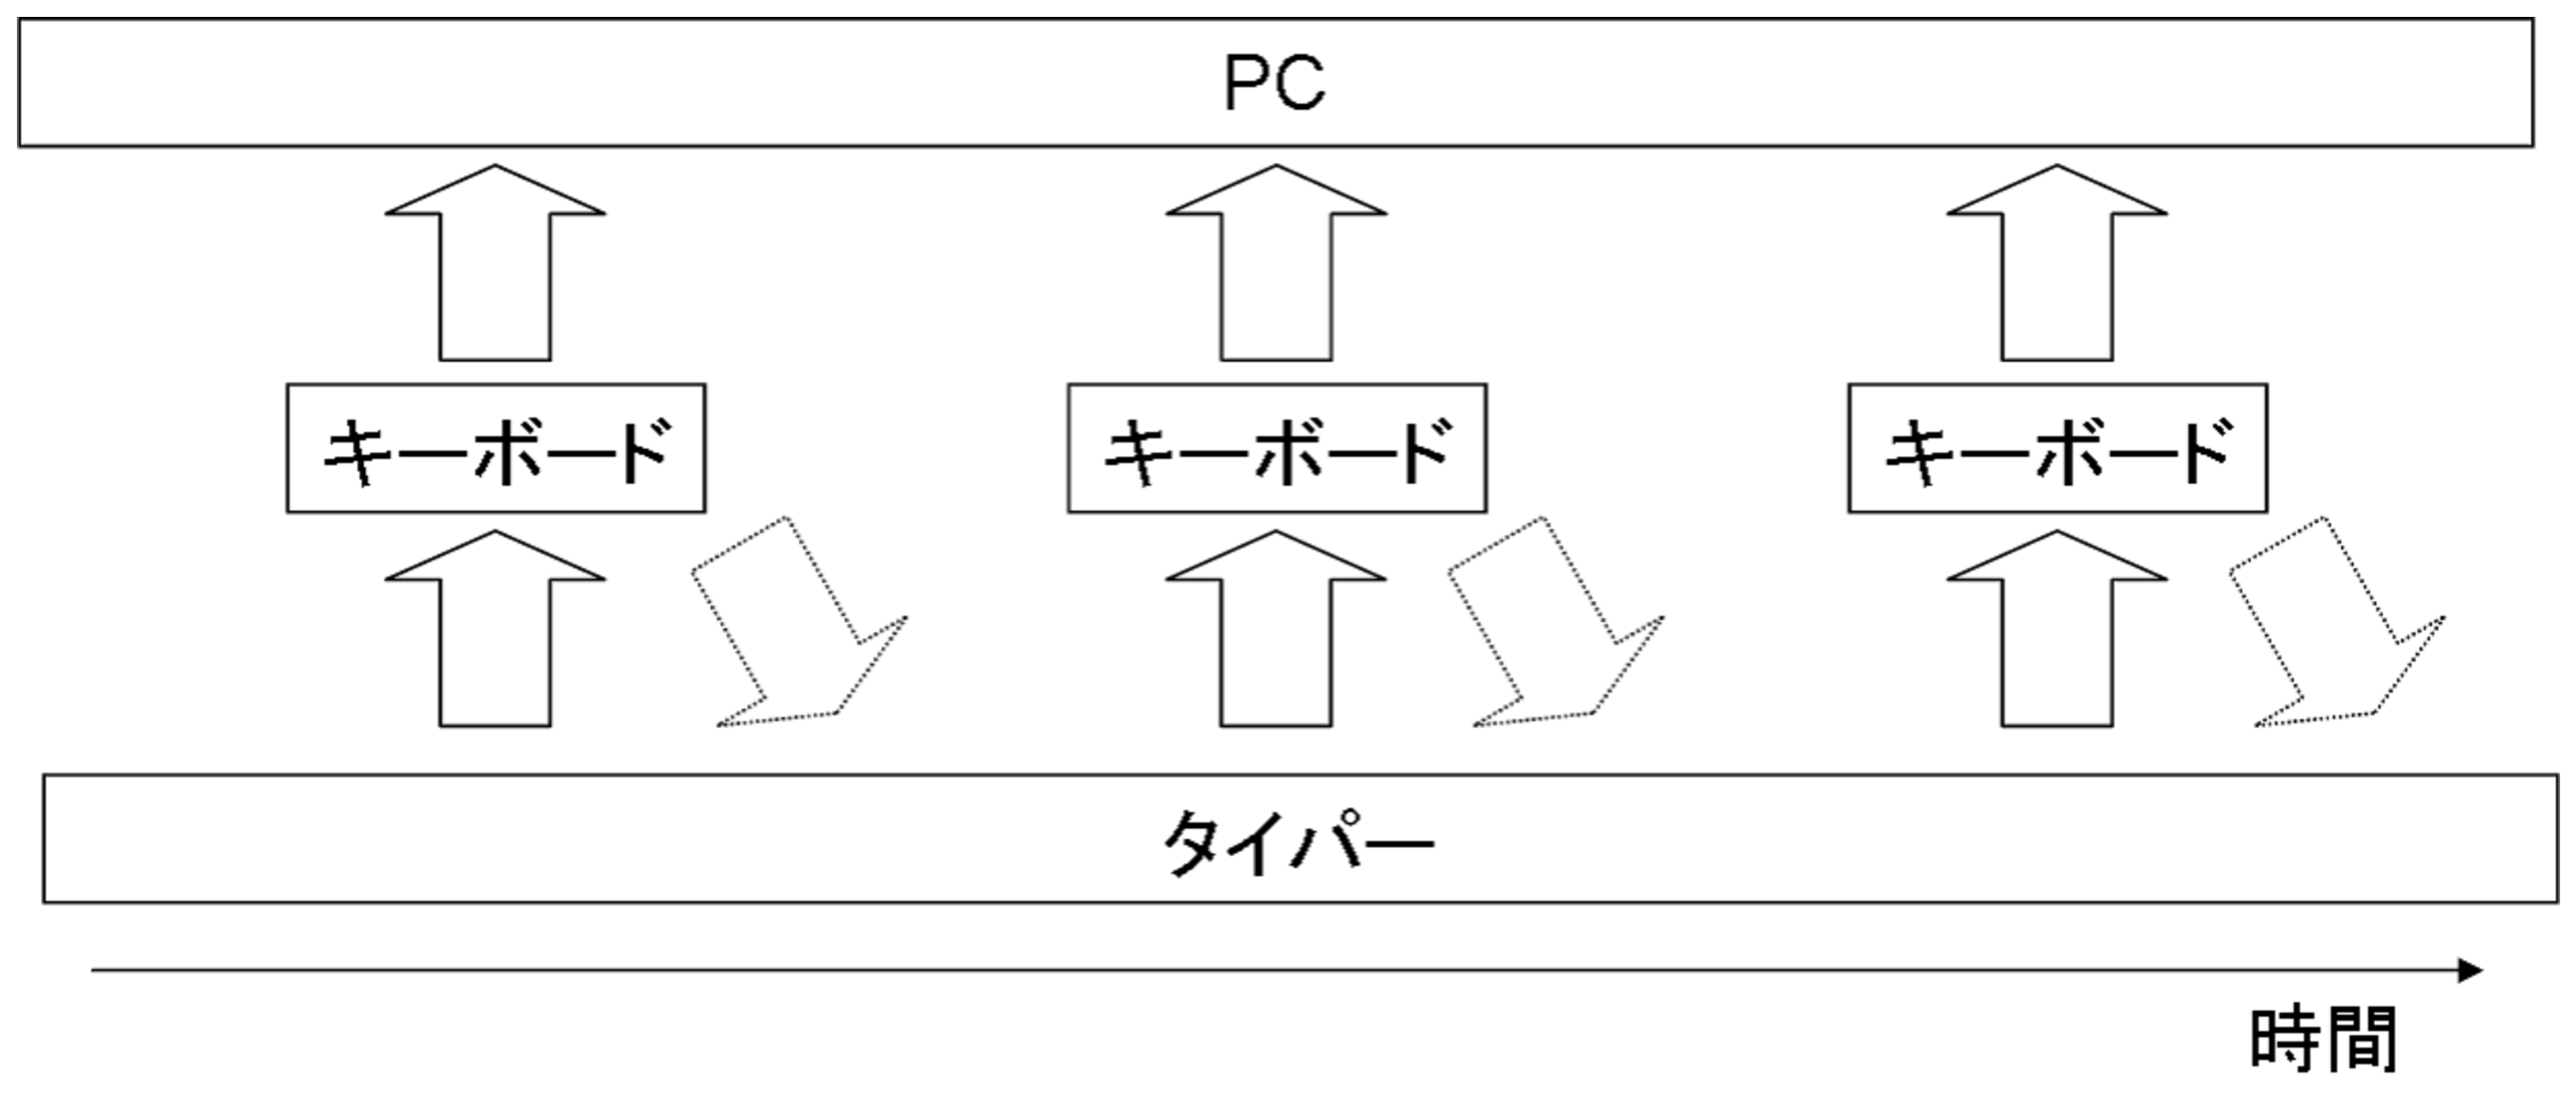
\includegraphics[width=14cm,clip]{res_eigh/img6.eps}
 \end{center}
 \caption{キーボードからの入力を無視して打つスタイル}
 \label{eigh:img6}
\end{figure*}

\begin{figure*}
 \begin{center}
   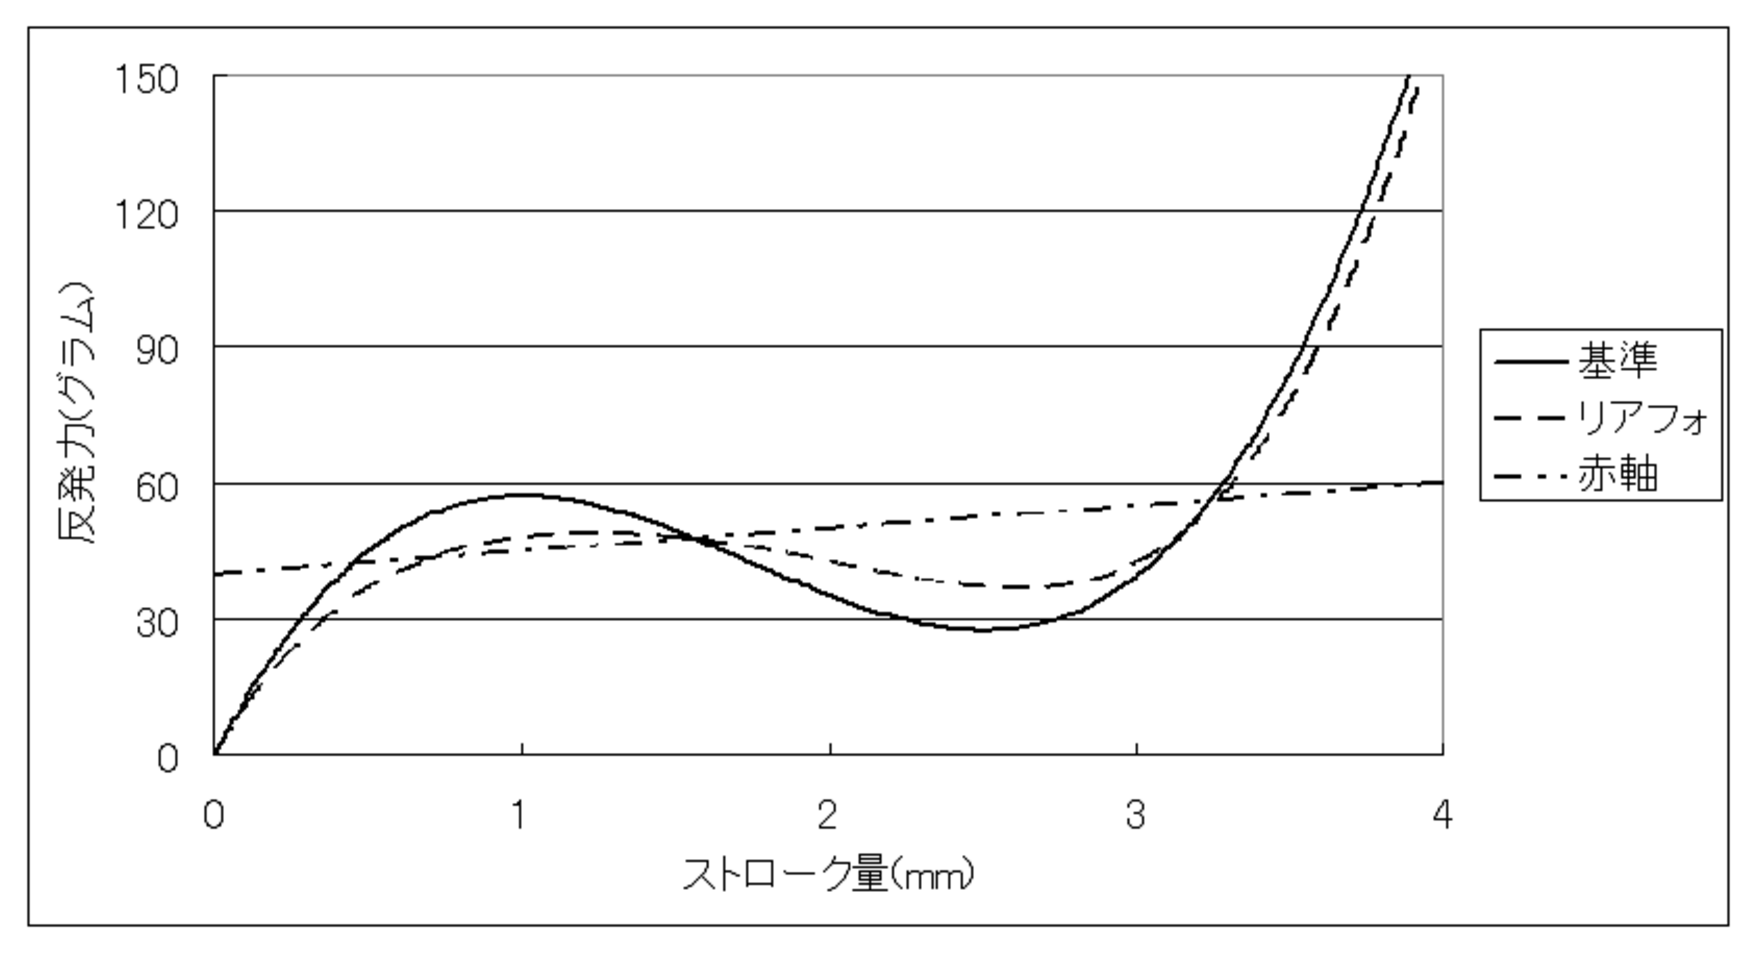
\includegraphics[width=14cm,clip]{res_eigh/img7.eps}
 \end{center}
 \caption{キーボードごとの荷重特性の違い}
 \label{eigh:img7}
\end{figure*}

\subsection{まとめ}
速いキーボードの特徴として「入力に要する時間」と「入力の強さ」から考えてみました。個人的にはこの2つの特徴で「反応がいいキーボード」と「邪魔されにくいキーボード」としています。これらは完全に両立するものではなく別の種類として考えています。人によってどちらが向いているかは違ってくると思います。自分のタイピングの特徴なども考慮しつつ、これらの特徴に注目すると良いキーボードが選べるかもしれません。

\section{打ち方とキーボード}

\subsection{パンタの特権?スライド打鍵}
パンタ特有の打ち方としてスライド打鍵と呼ばれるものがあります。これは押し込んだ指を戻さず次のキーへすべらせて打つ方法です(図\ref{eigh:img8})。打ってから戻るという動きがなくなり、その分次の動作に早く移ることができるため速く打つことができます。パンタでは短いストロークとキートップの形状によってこのスライドが非常にやりやすくなっています。実際には図のような複数の動作としてではなく、1回の動作としてやっていると思います。

\begin{figure*}
 \begin{center}
   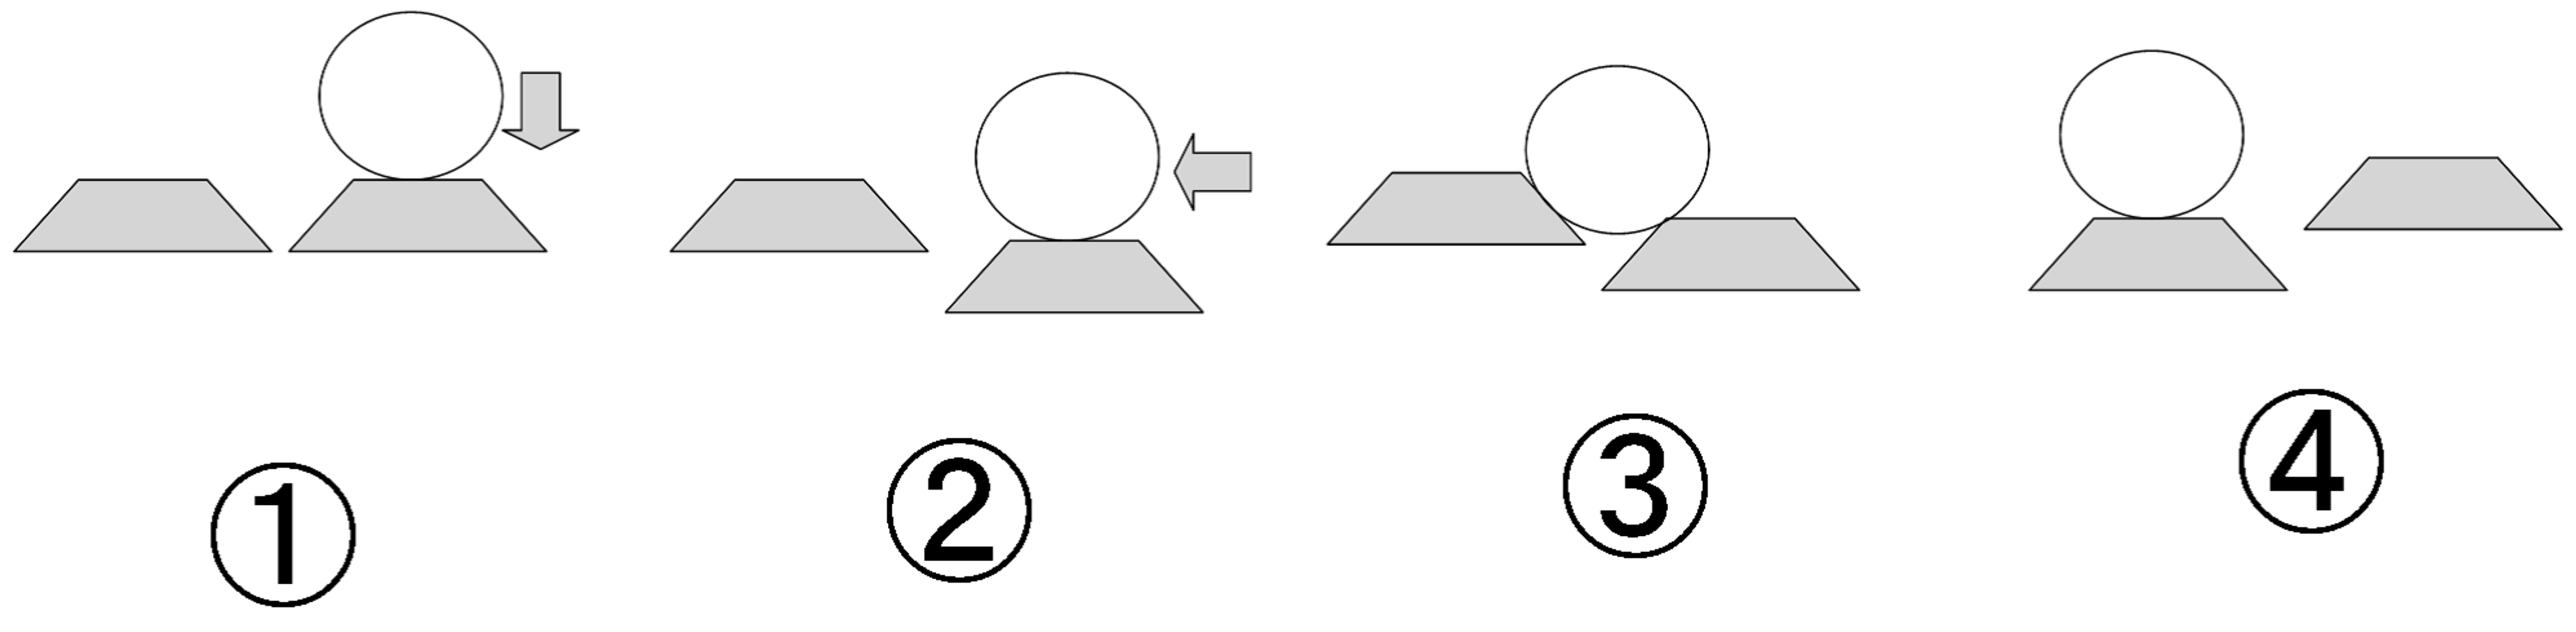
\includegraphics[width=14cm,clip]{res_eigh/img8.eps}
 \end{center}
 \caption{スライド打鍵}
 \label{eigh:img8}
\end{figure*}

\subsection{軽いと指だけで打てる?}
キーの軽さというのは重要な要素ですが打ち方に対してどのような影響があるでしょうか。個人的には指だけで打てるというのがあります。重いキーボードではどうしても手の力も使ってしまうために同じ手が連続するような場面ではどうしても手の動きにより指の動きが制限されやすくなります。一方、指の力のみで押せるような軽いキーボードでは片手に集中するような場面でも手全体の動きに制限されにくく、このような場面でも速く打てるのではないでしょうか。

\subsection{まとめ}
キーボードによる打ち方の違いは、特定のキーボードだと特定の打ち方ができる、というよりは、ある条件下では特定の打ち方ができないと言ったものになっています。キーボードによって打ち方に制限が生まれ、速さや成長に影響しているかもしれません。

\section{改造してみよう}
キーボードは少し(?)の改造で驚くほど打鍵感が変わったりします。いくつか例を挙げたいと思います。 必ずしも速く打てるようになるとは限りませんが試してみるのもいいかもしれません。

\subsection{下に何かを敷いてみる}
キーボードの下に何か挟んでみます。挟む場所や物等によって結構打鍵感が変わります。おすすめは入手も簡単な滑り止めシートでしょうか。無駄な振動が減ってなめらかに打てるようになるような気がします。その他にも手前部分のみに本を挟みキーボードの角度を変える方法も試してみて欲しいです。慣れないと打ちにくいかもしれませんが、場合によっては打ちやすくなるかもしれません。いずれにせよ打ちにくくても戻せばいいだけなのでどんどん試してみましょう。

\subsection{荷重を軽くする}

\subsubsection*{ラバードームに切込みを入れる}
これをやってしまうと元に戻すことはできませんが、軽いキーボードが欲しい場合には試してみるのもいいかもしれません。方法は分解後にラバードームに2、3ヶ所切り込みを入れていくだけです。切り方などにもよりますが結構変わります。ただ、重さやスイッチがオンになる場所にばらつきが出てしまうためあまりお勧めしません。改造自体を目的としてやってみるのもありかもしれません。

\subsubsection*{ラバードームを潰したままの状態で放置する}

キーボードの上におもりなどを乗せ、キーが押された状態のまましばらく(数時間から1日程度)放置します。放置後にはラバードームの反発力が弱くなります。
実際に試したのは1個だけですが実際軽くなったような気がします。これをやっていない部分に比べてやった部分のキーでは明らかに軽くなっています。ばらつきが激しかったり分解が面倒だったりするラバードームを切る方法と比べるとこちらがおすすめです。

\subsection{ストロークを短くする}
キートップと本体の間に何かを挟み(図\ref{eigh:img9})ストロークを短くします。場合によってはキートップを再び付けられなくなったりするので、挟み方や材質などは制限されてしまいます。色々工夫してみるのもいいかもしれません。

\begin{figure*}
 \begin{center}
   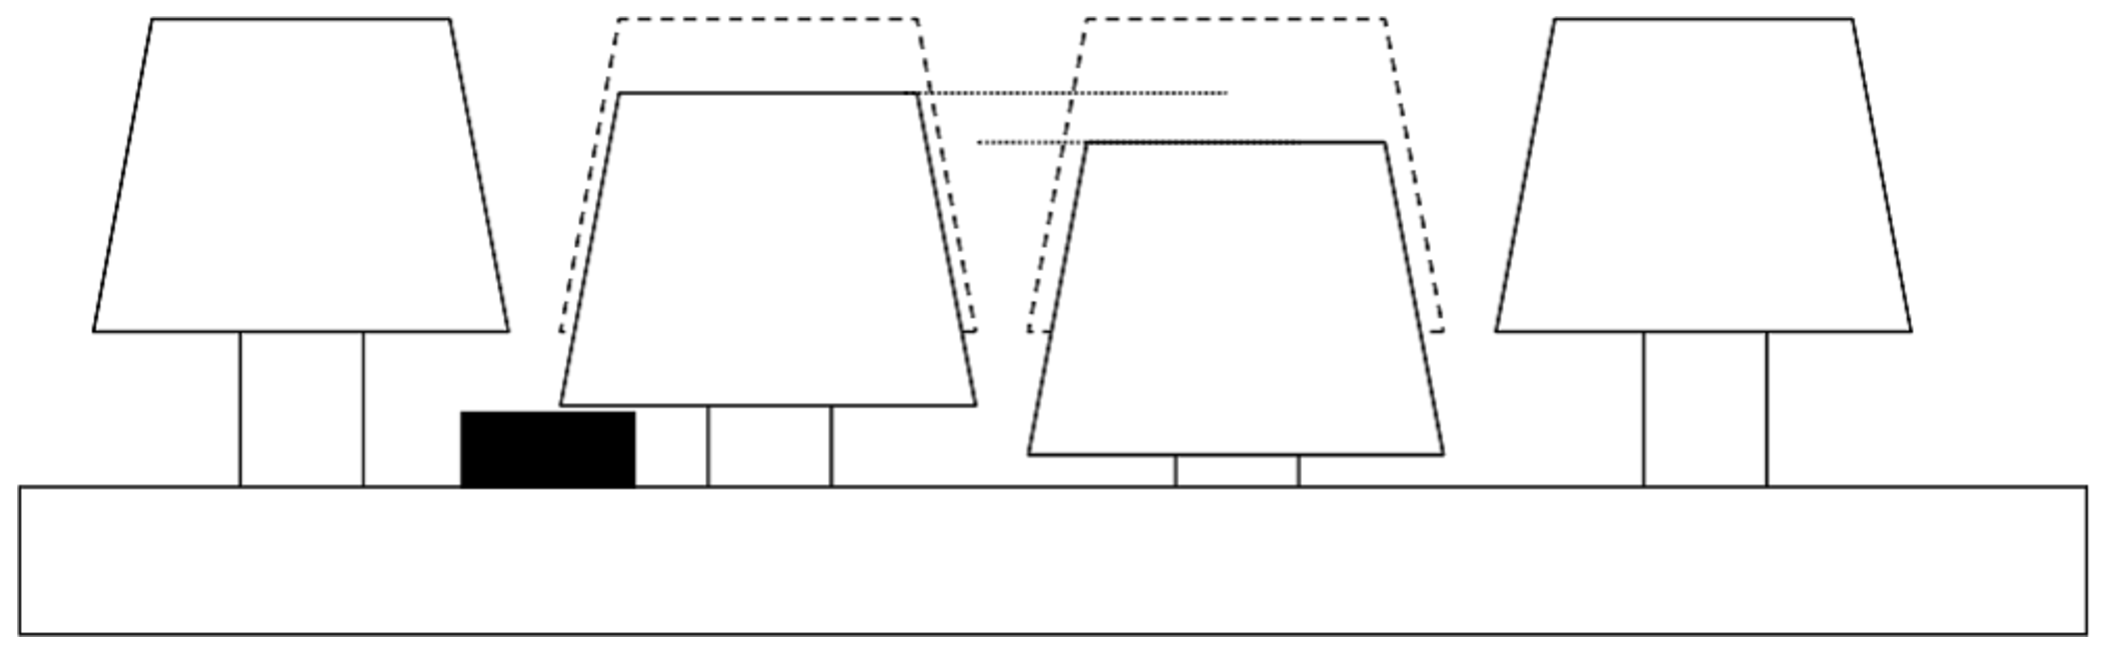
\includegraphics[width=14cm,clip]{res_eigh/img9.eps}
 \end{center}
 \caption{キートップと本体の間に挟む}
 \label{eigh:img9}
\end{figure*}


\section{キーボードとのつきあいかた}
ここではキーボードの選び方や使い方を十数個のキーボードを打ってきた経験に基づいて色々書いていこうと思います。

\subsection{お勧めのキーボード教えて?}
打ち方など個人に依存することが大きいので単純におすすめを挙げることはできません。パンタ以外でおすすめを挙げるとするとやはりリアフォを選ぶのが無難だと思います。記録を出す手段としてのキーボード選びという事ならば、安いものをいくつも試すよりリアフォを買ってしまったほうがいいと思います。なかなか壊れませんし同時押しの問題が発生することが無いのでそれほど高い買い物にはならないでしょう。一方パンタでのおすすめというとちょっと答えにくいです。logicoolのCZ-900は人気があり非常に良いキーボードだと思うのですが、パンタとしてはやや深めのストロークで有ることから特にスライド打鍵などで打ちにくさを感じることが多いようです。とはいえ、初めてのパンタとして使うには比較的使いやすいという意見も多いのでおすすめです。


\subsection{リアフォってたくさん種類あるけどどれ選んだらいいの?}
テンキーの有無や色については好みで選べばいいでしょう。問題は荷重ですが現在売っているものは3種類あります(過去にAll55gのものも限定販売されてました)。All45gの物と30gのもの、小指以外が45gで小指の部分が30gの変荷重があります。他のキーボードを使う場合やタイピングのスタイルによって合っているものが変わってくると思います。

\subsubsection*{変荷重}
そこそこお勧めです。力の弱い小指部分が軽くなっており、そこがいい部分であり、悪い部分であると言えます。小指の部分が他の指の部分と感覚が異なるためキーボードからの入力が指によって異なり、リズムが取りにくくなるかもしれません。また、軽いキーに慣れてしまうため小指の力が衰え、他のキーボードを打つ場合に小指部分だけ押せてないミスが発生することが多くなります。小指以外で小指キーを担当する場合もその部分だけ特性が違うため、慣れないうちは戸惑うことになるかもしれません。また、小指の担当キーでも\key{Shift}キーは45gなので注意が必要です。

\subsubsection*{All45g}
個人的にはこれがお勧めです。小指部分も同じ荷重のため特性の違いによる感覚の違いもなく、小指の劣化という問題もありません。変荷重になれた人は小指が重いと感じることもあるようです。

\subsubsection*{All30g}
とにかく軽いです。別物と言ってもいいと思います。キーを打つと言うよりキーの位置で指を動かすことで入力ができるような感覚です。軽すぎるために慣れないうちはかすりミスが大量発生するらしいです。反発力が弱いため、指の位置を戻すための動作が必要なのか、軽いけど他より疲れるという人もいるようです。


\subsection{メカニカルキーボードってどうなの?}
メカニカルキーボードは、ラバードームを使ったものとは結構荷重特性が違ったりするのである程度慣れが必要だとは思います。メカニカルキーボードはメンブレンシートを使ったものよりも同時押しの問題が発生しにくいのでその部分でのアドバンテージはあります。ただメカニカルキーボードといってもスイッチの違いなど様々なものがあります。また、同じスイッチを使っていても結構打鍵感が違ってくるので注意しましょう。「同じスイッチ=同じ打鍵感」と思っていると結構驚くことは多いかもしれません。これはラバードーム+メンブレンでも打鍵感が様々であるのと同じですね。

\subsection{複数のキーボードを使い分けるメリットは?}
まず、「いろんな感覚を味わえて楽しい」という点を挙げられます。これは人それぞれだとは思いますが、キーボードの打ち分けによる感覚の違いや打ち方の変化を楽しむという楽しみ方も面白いと思います。

2つ目に「キーボードによってタイピングが変わる」ということでしょうか。例えばリアフォに慣れるとそれぞれの指を独立して動かすような打ち方ができるようになってきます。そのため、リアフォから他のキーボードに行ったときに指で打つという感覚で打てるようになることがあります(私の場合はその効果はずっと続くわけではないです)。小指が軽いリアフォに慣れることで「小指が動きにくくなる」という悪い部分もあったりしますが複数のキーボードを使い分けることで打ち方が変化し、ある能力の向上に役立つこともあると思います。

3つ目としては競技ごとに使い分けられるということです。例えば長文を打つタイプウェル憲法では疲れにくいリアフォ、ミス減点が多いe-typingでは他のキーボードと言った使い分けができることです。
他には壊れてもすぐにタイピングができなくなるわけではないということでしょうか。まあ押入れに予備を入れておくとか他の方法はありますが……。

\subsection{リアフォって個体差大きくない?}
なぜかリアフォ使用者が他の人のリアフォを使うと「なんか自分のやつと打鍵感違う」と感じることが多いようです。使い込みによってラバードームが柔らかくなるため、人によってよく使うキーが違うために出るのではと言われたりもします。店で打った感じでも結構昔から置いてある店と比較的最近から置いてある店の物は打鍵感が違うようには感じます。個人的には使い込んだリアフォのほうが打ちやすいと思います。というか僕のリアフォ打ちにくいです。これは打ち込みが足りないからなんでしょうか?

\subsection{アイソレーションタイプのキーボードってどう?}
最近ノートPCに採用が増えてきたアイソレーションタイプ。本体の剛性をあげられるためより薄く、小さく、軽く作れるようになるらしいです。タイパーとして見ると特に下段でよくキーの間を叩いてしまうミスが発生しやすいです。巻き込みミスは減ってもうまく叩けないことによる詰まりミスが発生してミスが増えることもあると思います。普通のパンタと比べるとスライドしにくい、巻き込みミスをしにくい、慣れないと詰まりミスが出やすいといった特徴があります。

\subsection{実力を上げるためにあえて使いにくいキーボードで練習するのはどう?}
記録狙いのキーボードとの併用はありかもしれませんが、打ちにくいキーボードだけで練習するのはお勧めできません。これは個人的な体験なのですが打ちにくいキーボードに替えた途端成長が止まった事がありました。これはこの本の記事の一つであるタイピング練習論から言葉を借りると、動作速度が制限されたことで認識速度や組み立て速度が常に余裕がある状態になり、それらが成長しない状況に陥っていたためだと考えられます。タイピングに必要な指の運動能力は強さではなく速さだと思います。この能力は打ちやすいキーボードを使うことで身につけるべきだと思います。個人的には打ちやすいキーボードで動作速度のボトルネックを減らしたほうが他の能力の向上、全体的な実力の向上につながると考えています。

\subsection{ところでどんなキーボード使ってるの?}
今所有してるのは10個程度ですが実際にタイピングで使っているのは5個くらいです。その中でも記録を狙うような場合に使っているのはリアフォとCZ-900です。気分や種目によってその2つを使い分けています。その他にも遊び半分でメカニカル、正確性の練習でアイソレーションタイプのキーボードを使っています。

\section{おわりに}
私はキーボード選びはあくまでも記録を伸ばすための手段の一つだと思っています。記録を伸ばす手段としてキーボードを購入しているうちに所持数が増えてしまいました。これまで色々なキーボードを打ってきた中で、速く打てるキーボードには3章で挙げた2つの特徴である「反応の良さ」と「邪魔されにくさ」があると感じています。新しくキーボードを買うときもこの2つの特徴に注目して選んでいます。

また、キーボードは打ち方にも影響を与え、タイパーを変化させる要素にもなっていると思います。自分自身もキーボードを替えたことでここまで記録が伸びたと思っています。

いろんな種類のキーボードを打って色々な違いを楽しんだり、キーボードによって起こる自分のタイピングの変化を感じるのも楽しいですよ。
この記事がタイパーが一度キーボードについて考えなおす機会になり、キーボードを通してよりタイピングが楽しめるようになればと思います。

多くのタイパーがより良いキーボードに巡り合えることを願っています。
